\documentclass[conference]{IEEEtran}
\IEEEoverridecommandlockouts

% Packages
\usepackage{cite}
\usepackage{amsmath,amssymb,amsfonts}
\usepackage{algorithmic}
\usepackage{graphicx}
\usepackage[utf8]{inputenc}
\usepackage{textgreek}
\usepackage{textcomp}
\usepackage{xcolor}
\usepackage{listings}
\usepackage{caption}
\usepackage{subcaption}
\usepackage{booktabs}
\usepackage{multirow}
\usepackage{array}
\usepackage{float}

% Bibliography formatting
\def\BibTeX{{\rm B\kern-.05em{\sc i\kern-.025em b}\kern-.08em
    T\kern-.1667em\lower.7ex\hbox{E}\kern-.125emX}}

\author{
\IEEEauthorblockN{Siddhant Shah (B23334)\textsuperscript{*}, 
                  Aman (T25121)\textsuperscript{†}, 
                  Omkar Sharan (T25132)\textsuperscript{‡}}
\IEEEauthorblockA{\textsuperscript{*}b23334@students.iitmandi.ac.in \\
                  \textsuperscript{†}t25121@students.iitmandi.ac.in \\
                  \textsuperscript{‡}t25132@students.iitmandi.ac.in}
}

\begin{document}

% ================= TITLE =================
\title{Experiment: 2\\Analysis of Common Source Amplifier Circuits: DC, Transient, and AC Characterization Across Process Corners}

\maketitle

% ================= ABSTRACT =================
\begin{abstract}
\noindent
This study presents a comprehensive characterization of five common source amplifier circuits through DC, transient, and AC analyses using Cadence simulations. Circuit 1 undergoes full corner analysis across TT, FF, SS, SF, and FS conditions, revealing gain variations from 6.90 dB to 11.95 dB in AC analysis and 9.47 dB to 11.1 dB in transient analysis. Circuits 2-5 are analyzed at the TT corner, achieving AC gains of 4.95 dB, 25.9 dB, 23.76 dB, and 12.67 dB respectively. DC bias voltages are optimized at 700 mV for all circuits, with additional bias points ranging from 600 mV to 1.02 V for multi-stage configurations. The analysis demonstrates significant process-dependent performance variations while maintaining consistent 180° phase inversion across all topologies, establishing design margins essential for robust analog circuit implementation.
\end{abstract}

% ================= KEYWORDS =================
\begin{IEEEkeywords}
Common Source Amplifier, Process Corners, MOSFET, AC Analysis, Transient Analysis, cadence Simulation
\end{IEEEkeywords}

% ================= INTRODUCTION =================
\section{Introduction}  
\noindent  
The common source (CS) amplifier is a key element in analog IC design, widely employed for voltage amplification due to its high gain and moderate input impedance \cite{razavi}. In a MOSFET-based CS stage, the input is applied at the gate, the source is usually grounded, and the output is taken from the drain. Operation in the saturation region ensures linear amplification with an inverted output \cite{gray}.  

\noindent  
The small-signal gain is mainly governed by the MOSFET transconductance (\(g_m\)) and the load resistance (\(R_L\)), given by \cite{johns}:  
\[
A_v = -g_m R_L
\]  
where the negative sign indicates phase inversion.  

\noindent  
Since device parameters vary with manufacturing processes, circuit performance must be verified across process corners—TT, FF, SS, SF, and FS \cite{carusone}. Such analysis helps ensure that the amplifier remains reliable under different fabrication conditions.  

\noindent  
This study compares five CS amplifier variants in terms of DC biasing, transient behavior, and frequency response to evaluate their performance and robustness.  
evaluation.

% ================= DESIGN METHODOLOGY =================
\section{Theoretical Expressions for DC Operating Points, Small-Signal Gain, and Frequency Response}

\subsection{DC Analysis}
\noindent
The DC bias voltages and small-signal resistance can be expressed as \cite{razavi}:
\begin{equation}
    V_B = V_{GS} - V_{th}, \qquad 
    R_D = \frac{V_{DD} - V_{DS}}{I_D}
    \label{eq:dc}
\end{equation}
\noindent
The DC operating point of each circuit is determined to extract bias voltages ($V_B$) and equivalent resistances ($R_D$) \cite{gray}.  
The values are presented in tables for each circuit.

\subsection{Transient Analysis}
\noindent
For a sinusoidal input $v_{in}(t)$, the output amplitude is measured in the time domain.  
The small-signal voltage gain is the amplitude ratio \cite{johns}:
\begin{equation}
    A_v = \frac{V_{out,\;peak}}{V_{in,\;peak}}
    \label{eq:gain}
\end{equation}
which may also be expressed in decibels (dB) as:
\begin{equation}
    \text{Gain (dB)} = 20 \log_{10}(A_v)
    \label{eq:gain_dB}
\end{equation}
\noindent
The phase shift is calculated from the relative delay between input and output waveforms \cite{gray}.  

\noindent
Transient simulations are performed by applying a sinusoidal input signal. The input and output waveforms are plotted with respect to time.  
This analysis is repeated across all process corners — Typical-Typical (TT), Fast-Fast (FF), Slow-Slow (SS), Slow-Fast (SF), and Fast-Slow (FS) but only for circuit 1. For rest all circuits the analysis is repeated only across Typical-Typical (TT) corners.
The plots of $V_{in}$ and $V_{out}$ vs. time are presented for the TT corner, while the gain and phase shift values for all corners (Q1) and TT (other questions) are summarized in tables.

\subsection{AC Analysis}
\noindent
The frequency response is obtained from small-signal AC analysis, where the transfer function is \cite{carusone}:
\begin{equation}
    A_v(j\omega) = \frac{V_{out}(j\omega)}{V_{in}(j\omega)}
    \label{eq:tf}
\end{equation}
\noindent
The magnitude is conventionally plotted in decibels (dB), and the phase in degrees.  
The unity-gain bandwidth (UGB) is the frequency where the magnitude equals 0~dB \cite{razavi}.  
The phase margin (PM) is defined as \cite{gray}:
\begin{equation}
    PM = 180^{\circ} + \angle A_v(j\omega_{UGB})
    \label{eq:pm}
\end{equation}
\noindent
Small-signal AC analysis is carried out to determine the frequency response. Magnitude and phase plots are generated for each circuit \cite{johns}.  
As in the transient case, the analysis is performed across all process corners (TT, FF, SS, SF, FS).  
\noindent
The Bode plots (magnitude vs. frequency and phase vs. frequency) are shown for the TT corner, and the tabulated results report gain and phase margin for TT.


% ================= CIRCUIT 1 =================
\section{Circuit 1: Basic Common Source Amplifier}

% \subsection{Schematic}
\begin{figure}[H]
    \centering
    \includegraphics[width=0.40\textwidth, height=0.35\textwidth]{ckt1.eps}
    \caption{Circuit 1 Schematic}
    \label{fig:circuit1}
\end{figure}

% \subsection{DC Analysis}
\noindent
The DC analysis determines the optimal bias conditions for proper amplifier operation \cite{razavi}.

\begin{table}[H]
    \centering
    \caption{DC Analysis Results for Circuit 1}
    \begin{tabular}{|c|c|}
        \hline
        \textbf{Parameter} & \textbf{Value} \\
        \hline
        Bias Voltage (\(V_b\)) & 700 mV \\
        \hline
        Output Resistance (\(R_o\)) & 6.33 k\(\Omega\) \\
        \hline
    \end{tabular}
    \label{tab:dc1}
\end{table}

% \subsection{Transient Analysis}
\noindent
Transient analysis evaluates the time-domain response across different process corners \cite{johns}.

\begin{table}[H]
    \centering
    \caption{Transient Analysis Results for Circuit 1}
    \begin{tabular}{|c|c|c|}
        \hline
        \textbf{Corner} & \textbf{Gain (dB)} & \textbf{Phase (°)} \\
        \hline
        TT & 10.09 & 180 \\
        \hline
        FF & 11.1 & 180 \\
        \hline
        SS & 9.47 & 180 \\
        \hline
        SF & 11.1 & 180 \\
        \hline
        FS & 11.1 & 180 \\
        \hline
    \end{tabular}
    \label{tab:transient1}
\end{table}

\begin{figure}[H]
    \centering
    \includegraphics[width=0.5\textwidth, height=0.35\textheight]{q1_tran_tt.png}
    \caption{Transient Analysis for Circuit 1 – TT Corner}
    \label{fig:c1_trans_tt}
\end{figure}

% \begin{figure}[H]
%     \centering
%     \includegraphics[width=0.45\textwidth]{q1_tran_ff.png}
%     \caption{Transient Analysis for Circuit 1 – FF Corner}
%     \label{fig:c1_trans_ff}
% \end{figure}

% \begin{figure}[H]
%     \centering
%     \includegraphics[width=0.45\textwidth]{q1_tran_ss.png}
%     \caption{Transient Analysis for Circuit 1 – SS Corner}
%     \label{fig:c1_trans_ss}
% \end{figure}

% \begin{figure}[H]
%     \centering
%     \includegraphics[width=0.45\textwidth]{q1_tran_sf.png}
%     \caption{Transient Analysis for Circuit 1 – SF Corner}
%     \label{fig:c1_trans_sf}
% \end{figure}

% \begin{figure}[H]
%     \centering
%     \includegraphics[width=0.45\textwidth]{q1_tran_fs.png}
%     \caption{Transient Analysis for Circuit 1 – FS Corner}
%     \label{fig:c1_trans_fs}
% \end{figure}

% \subsection{AC Analysis}
\noindent 
AC analysis characterizes the frequency response and determines the gain-bandwidth product \cite{gray}.

\begin{table}[H]
    \centering
    \caption{AC Analysis Results for Circuit 1}
    \begin{tabular}{|c|c|c|}
        \hline
        \textbf{Corner} & \textbf{Gain (dB)} & \textbf{Phase (°)} \\
        \hline
        TT & 10.415 & 180 \\
        \hline
        FF & 11.9477 & 180 \\
        \hline
        SS & 6.90179 & 180 \\
        \hline
        SF & 8.96632 & 180 \\
        \hline
        FS & 11.3679 & 180 \\
        \hline
    \end{tabular}
    \label{tab:ac1}
\end{table}

\begin{figure}[H]
    \centering
    \includegraphics[width=0.55\textwidth, height=0.35\textheight]{q1_ac_tt.png}
    \caption{AC Analysis for Circuit 1 – TT Corner}
    \label{fig:c1_ac_tt}
\end{figure}

% \begin{figure}[H]
%     \centering
%     \includegraphics[width=0.45\textwidth]{q1_ac_ff.png}
%     \caption{AC Analysis for Circuit 1 – FF Corner}
%     \label{fig:c1_ac_ff}
% \end{figure}

% \begin{figure}[H]
%     \centering
%     \includegraphics[width=0.45\textwidth]{q1_ac_ss.png}
%     \caption{AC Analysis for Circuit 1 – SS Corner}
%     \label{fig:c1_ac_ss}
% \end{figure}

% \begin{figure}[H]
%     \centering
%     \includegraphics[width=0.45\textwidth]{q1_ac_sf.png}
%     \caption{AC Analysis for Circuit 1 – SF Corner}
%     \label{fig:c1_ac_sf}
% \end{figure}

% \begin{figure}[H]
%     \centering
%     \includegraphics[width=0.45\textwidth]{q1_ac_fs.png}
%     \caption{AC Analysis for Circuit 1 – FS Corner}
%     \label{fig:c1_ac_fs}
% \end{figure}

% ================= CIRCUIT 2 =================
\section{Circuit 2: Common Source Amplifier Variant}

% \subsection{Schematic}
\begin{figure}[H]
    \centering
    \includegraphics[width=0.40\textwidth, height=0.35\textwidth]{ckt2.eps}
    \caption{Circuit 2 Schematic}
    \label{fig:circuit2}
\end{figure}

% \subsection{DC Analysis}
\begin{table}[H]
    \centering
    \caption{DC Analysis Results for Circuit 2}
    \begin{tabular}{|c|c|}
        \hline
        \textbf{Parameter} & \textbf{Value} \\
        \hline
        Bias Voltage (\(V_b\)) & 700 mV \\
        \hline
    \end{tabular}
    \label{tab:dc2}
\end{table}

% \subsection{Transient Analysis}
\begin{table}[H]
    \centering
    \caption{Transient Analysis Results for Circuit 2 (TT Corner)}
    \begin{tabular}{|c|c|c|}
        \hline
        \textbf{Corner} & \textbf{Gain (dB)} & \textbf{Phase (°)} \\
        \hline
        TT & 4.76 & 180 \\
        \hline
    \end{tabular}
    \label{tab:transient2}
\end{table}

\begin{figure}[H]
    \centering
    \includegraphics[width=0.5\textwidth, height=0.35\textheight]{q2_tran_tt.png}
    \caption{Circuit 2 Transient Analysis (TT Corner)}
    \label{fig:transient2}
\end{figure}

% \subsection{AC Analysis}
\begin{table}[H]
    \centering
    \caption{AC Analysis Results for Circuit 2 (TT Corner)}
    \begin{tabular}{|c|c|c|}
        \hline
        \textbf{Corner} & \textbf{Gain (dB)} & \textbf{Phase (°)} \\
        \hline
        TT & 4.94875 & 179.99 \\
        \hline
    \end{tabular}
    \label{tab:ac2}
\end{table}

\begin{figure}[H]
    \centering
    \includegraphics[width=0.55\textwidth,height=0.35\textheight]{q2_ac_tt.png}
    \caption{Circuit 2 AC Analysis (TT Corner)}
    \label{fig:ac2}
\end{figure}

% ================= CIRCUIT 3 =================
\section{Circuit 3: Enhanced Common Source Amplifier}

% \subsection{Schematic}
\begin{figure}[H]
    \centering
    \includegraphics[width=0.45\textwidth, height=0.4\textwidth]{ckt3.eps}
    \caption{Circuit 3 Schematic}
    \label{fig:circuit3}
\end{figure}

% \subsection{DC Analysis}
\begin{table}[H]
    \centering
    \caption{DC Analysis Results for Circuit 3}
    \begin{tabular}{|c|c|}
        \hline
        \textbf{Parameter} & \textbf{Value} \\
        \hline
        Bias Voltage (\(V_b\)) & 0.7 V \\
        \hline
        \(V_{b2}\) & 0.8 V \\
        \hline
    \end{tabular}
    \label{tab:dc3}
\end{table}

% \subsection{Transient Analysis}
\begin{table}[H]
    \centering
    \caption{Transient Analysis Results for Circuit 3 (TT Corner)}
    \begin{tabular}{|c|c|c|}
        \hline
        \textbf{Corner} & \textbf{Gain (dB)} & \textbf{Phase (°)} \\
        \hline
        TT & 17.68 & 180 \\
        \hline
    \end{tabular}
    \label{tab:transient3}
\end{table}

\begin{figure}[H]
    \centering
    \includegraphics[width=0.5\textwidth, height=0.35\textheight]{q3_tran_tt.png}
    \caption{Circuit 3 Transient Analysis (TT Corner)}
    \label{fig:transient3}
\end{figure}

% \subsection{AC Analysis}
\begin{table}[H]
    \centering
    \caption{AC Analysis Results for Circuit 3 (TT Corner)}
    \begin{tabular}{|c|c|c|}
        \hline
        \textbf{Corner} & \textbf{Gain (dB)} & \textbf{Phase (°)} \\
        \hline
        TT & 25.9 & 179.99 \\
        \hline
    \end{tabular}
    \label{tab:ac3}
\end{table}

\begin{figure}[H]
    \centering
    \includegraphics[width=0.5\textwidth, height=0.35\textheight]{q3_ac_tt.png}
    \caption{Circuit 3 AC Analysis (TT Corner)}
    \label{fig:ac3}
\end{figure}

% ================= CIRCUIT 4 =================
\section{Circuit 4: Advanced Common Source Configuration}

\subsection{Schematic}
\begin{figure}[H]
    \centering
    \includegraphics[width=0.45\textwidth, height=0.35\textwidth]{ckt4.eps}
    \caption{Circuit 4 Schematic}
    \label{fig:circuit4}
\end{figure}

\subsection{DC Analysis}
\begin{table}[H]
    \centering
    \caption{DC Analysis Results for Circuit 4}
    \begin{tabular}{|c|c|}
        \hline
        \textbf{Parameter} & \textbf{Value} \\
        \hline
        Bias Voltage (\(V_b\)) & 0.700 V \\
        \hline
        Voltage (\(V_{b2}\)) & 0.900 V \\
        \hline
        Source Resistance (\(R_s\)) & 3.07 k\(\Omega\) \\
        \hline
    \end{tabular}
    \label{tab:dc4}
\end{table}

\subsection{Transient Analysis}
\begin{table}[H]
    \centering
    \caption{Transient Analysis Results for Circuit 4 (TT Corner)}
    \begin{tabular}{|c|c|c|}
        \hline
        \textbf{Corner} & \textbf{Gain (dB)} & \textbf{Phase (°)} \\
        \hline
        TT & 17.61 & 180 \\
        \hline
    \end{tabular}
    \label{tab:transient4}
\end{table}

\begin{figure}[H]
    \centering
    \includegraphics[width=0.5\textwidth, height=0.25\textheight]{q4_tran_tt.png}
    \caption{Circuit 4 Transient Analysis (TT Corner)}
    \label{fig:transient4}
\end{figure}

\subsection{AC Analysis}
\begin{table}[H]
    \centering
    \caption{AC Analysis Results for Circuit 4 (TT Corner)}
    \begin{tabular}{|c|c|c|}
        \hline
        \textbf{Corner} & \textbf{Gain (dB)} & \textbf{Phase (°)} \\
        \hline
        TT & 23.76 & 180 \\
        \hline
    \end{tabular}
    \label{tab:ac4}
\end{table}

\begin{figure}[H]
    \centering
    \includegraphics[width=0.5\textwidth,height=0.35\textheight]{q4_ac_tt.png}
    \caption{Circuit 4 AC Analysis (TT Corner)}
    \label{fig:ac4}
\end{figure}

% ================= CIRCUIT 5 =================
\section{Circuit 5: Multi-Stage Common Source Amplifier}

% \subsection{Schematic}
\begin{figure}[H]
    \centering
    \includegraphics[width=0.45\textwidth,height=0.45\textwidth]{ckt5.eps}
    \caption{Circuit 5 Schematic}
    \label{fig:circuit5}
\end{figure}

% \subsection{DC Analysis}
\begin{table}[H]
    \centering
    \caption{DC Analysis Results for Circuit 5}
    \begin{tabular}{|c|c|}
        \hline
        \textbf{Parameter} & \textbf{Value} \\
        \hline
        Bias Voltage (\(V_b\)) & 0.7 V \\
        \hline
        Voltage (\(V_{b1}\)) & 0.6 V \\
        \hline
        Voltage (\(V_{b2}\)) & 1.02 V \\
        \hline
    \end{tabular}
    \label{tab:dc5}
\end{table}

% \subsection{Transient Analysis}
\begin{table}[H]
    \centering
    \caption{Transient Analysis Results for Circuit 5 (TT Corner)}
    \begin{tabular}{|c|c|c|}
        \hline
        \textbf{Corner} & \textbf{Gain (dB)} & \textbf{Phase (°)} \\
        \hline
        TT & 9.18 & 180 \\
        \hline
    \end{tabular}
    \label{tab:transient5}
\end{table}

\begin{figure}[H]
    \centering
    \includegraphics[width=0.5\textwidth, height=0.35\textheight]{q5_tran_tt.png}
    \caption{Circuit 5 Transient Analysis (TT Corner)}
    \label{fig:transient5}
\end{figure}

% \subsection{AC Analysis}
\begin{table}[H]
    \centering
    \caption{AC Analysis Results for Circuit 5 (TT Corner)}
    \begin{tabular}{|c|c|c|}
        \hline
        \textbf{Corner} & \textbf{Gain (dB)} & \textbf{Phase (°)} \\
        \hline
        TT & 12.6695 & 180 \\
        \hline
    \end{tabular}
    \label{tab:ac5}
\end{table}

\begin{figure}[H]
    \centering
    \includegraphics[width=0.5\textwidth, height=0.35\textheight]{q5_ac_tt.png}
    \caption{Circuit 5 AC Analysis (TT Corner)}
    \label{fig:ac5}
\end{figure}

% ================= DISCUSSION =================
\section{Discussion}
\noindent
The experimental investigation across five process corners (TT, FF, SS, SF, FS) for Circuit 1 revealed substantial performance disparities that underscore the critical importance of corner analysis in analog design verification \cite{carusone}. The Fast-Fast corner consistently delivered superior gain performance, achieving 11.95 dB in AC analysis compared to the Slow-Slow corner's 6.90 dB, representing a 5.05 dB variation. This significant deviation stems from enhanced carrier mobility and reduced threshold voltages under fast process conditions, which directly amplify the transconductance parameter and consequently boost overall amplification \cite{razavi}.

\noindent
The transient domain analysis exposed temporal characteristics that complement the frequency domain findings \cite{johns}. Circuit 1's transient gain variations from 9.47 dB to 11.1 dB across corners demonstrate process sensitivity in time-domain applications. The consistent 180° phase shift across all configurations validates the fundamental common-source inverting topology, confirming theoretical predictions regardless of process variations \cite{gray}.

\noindent
Among the circuit topologies evaluated, Circuit 3 emerged as the superior performer with 25.9 dB AC gain, attributed to its enhanced configuration incorporating additional bias control through $V_{b2} = 0.8$ V \cite{razavi}. This multi-bias approach enables optimized transistor operating points, maximizing transconductance utilization. Circuit 4 presented a balanced design philosophy, achieving 23.76 dB gain while maintaining reasonable complexity through its $V_{b2} = 0.9$ V biasing scheme and 3.07 kΩ source resistance integration.

\noindent
Interestingly, Circuit 5's multi-stage architecture yielded moderate gain (12.67 dB) despite its complex three-bias configuration ($V_b = 0.7$ V, $V_{b1} = 0.6$ V, $V_{b2} = 1.02$ V). This counterintuitive result suggests potential inter-stage loading effects or suboptimal bias distribution, highlighting the necessity for careful impedance matching in cascaded amplifier designs \cite{gray}.

% ================= CONCLUSION =================
\section{Conclusion}
\noindent
This comprehensive investigation successfully established quantitative performance metrics for five distinct common-source amplifier configurations through systematic DC, transient, and AC characterization methodologies \cite{johns}. The experimental framework demonstrated the profound influence of semiconductor manufacturing variations on circuit behavior, with Circuit 1 exhibiting gain fluctuations spanning nearly 5 dB across extreme process corners (6.90 dB to 11.95 dB) \cite{carusone}.

\noindent
The Fast-Fast process corner consistently emerged as the optimal performance condition, delivering maximum gain and bandwidth capabilities due to enhanced device characteristics \cite{razavi}. Conversely, the Slow-Slow corner established conservative performance boundaries, essential for worst-case design scenario validation. The asymmetric corners (SF and FS) provided intermediate performance levels, confirming the necessity of comprehensive corner verification in production-ready designs \cite{gray}.

\noindent
The implemented bias optimization strategy at 700 mV proved universally effective across all circuit variants, ensuring reliable saturation region operation regardless of topology complexity \cite{razavi}. The additional bias points ranging from 600 mV to 1.02 V in multi-stage configurations demonstrated the scalability of the biasing approach while maintaining operational stability.

\noindent
Circuit performance hierarchy emerged clearly from the analysis: Circuit 3 achieved exceptional amplification (25.9 dB AC gain) through optimized dual-bias architecture, Circuit 4 demonstrated balanced performance-complexity trade-offs (23.76 dB), while Circuit 2 provided minimal but stable gain (4.95 dB) suitable for specific low-gain applications. The multi-stage Circuit 5's moderate performance (12.67 dB) suggests opportunities for further optimization in cascaded topologies.

\noindent
The invariant 180° phase response across all configurations validates the theoretical foundation of common-source operation, providing confidence in the simulation methodology and design approach. This study establishes a robust framework for analog amplifier characterization that can be extended to other circuit families, contributing valuable insights for process-aware design methodologies in contemporary integrated circuit development.

% ================= REFERENCES =================
\begin{thebibliography}{9}
\bibitem{razavi}
B. Razavi, \textit{Design of Analog CMOS Integrated Circuits}, McGraw-Hill Education, 2nd Edition, 2016.

\bibitem{johns}
D. Johns and K. Martin, \textit{Analog Integrated Circuit Design}, John Wiley \& Sons, 2nd Edition, 2012.

\bibitem{gray}
P. Gray, P. Hurst, S. Lewis, and R. Meyer, \textit{Analysis and Design of Analog Integrated Circuits}, John Wiley \& Sons, 5th Edition, 2009.

\bibitem{carusone}
T. Carusone, D. Johns, and K. Martin, \textit{Analog Integrated Circuit Design}, John Wiley \& Sons, 2nd Edition, 2012.
\end{thebibliography}

\end{document}
